%\documentclass[xcolor=dvipsnames,10pt,handout]{beamer}
% ,handout
\documentclass[9pt]{beamer}
\usepackage{etex}

%\usepackage[francais]{babel}
\usepackage[utf8]{inputenc}
\usepackage{graphicx,pstricks,pst-node,pst-plot}
\usepackage{pxfonts} %concrete,pxfonts
\usepackage{charter} %mathptmx, newcent, charter
\usepackage[mathscr]{eucal}
\usepackage{multirow,epsfig}
\usepackage{pgf,pgflibraryshapes,pgflibraryarrows,tikz}  % old version
\usepackage{fancybox}
\usepackage{amsmath,amssymb,amsfonts,amsbsy,ifthen,rotate}
\usepackage{tabularx}
\usepackage{colortbl,xcolor}
\usepackage{setspace}
\usepackage{natbib}
\usepackage{tabularx,multirow}
\usepackage{slashbox}
\usepackage{graphicx}

\newcommand{\altx}{\usebeamercolor[fg]{alerted text}}
\newcommand{\titx}{\usebeamercolor[fg]{subtitle}}

\newcommand{\Variance}[2]{\mathbb{V}\text{ar}_{#1}\left[ #2 \right])}
\newcommand{\Expectation}[2]{\mathbb{E}_{#1}\left[ #2 \right]}
\newcommand{\N}[2]{\mathcal{N}\left( #1 , #2 \right)}
\newcommand{\PG}[2]{\mathrm{PG}\left( #1 , #2 \right)}
\newcommand{\VX}[1]{\mathrm{var}_X\left( #1 \right)}
\newcommand{\EX}[1]{\mathbb{E}_X\left[ #1 \right]}
\newcommand{\VZ}[1]{\mathrm{var}_Z\left( #1 \right)}
\newcommand{\covZ}[2]{\mathrm{cov}_Z\left( #1, #2 \right)}
\newcommand{\EZ}[1]{\mathbb{E}_Z\left[ #1 \right]}
\newcommand{\tX}{\tilde{X}}
\newcommand{\tx}{\tilde{x}}
\newcommand{\xnew}{x_{\mathrm{new}}}
\newcommand{\ynew}{y_{\mathrm{new}}}
\newcommand{\R}{\mathbb{R}}
\newcommand{\bbeta}{\boldsymbol{\beta}}
\newcommand{\aalpha}{\boldsymbol{\alpha}}
\newcommand{\nnu}{\boldsymbol{\nu}}
\newcommand{\DDelta}{\boldsymbol{\Delta}}
\newcommand{\ttheta}{\boldsymbol{\theta}}
\newcommand{\ff}{\textbf{f}}
\newcommand{\bb}{\textbf{b}}
\newcommand{\VV}{\textbf{V}}
\newcommand{\A}{\textbf{A}}
\newcommand{\RR}{\textbf{R}}
\newcommand{\rr}{\textbf{r}}
\newcommand{\z}{\textbf{z}}
\newcommand{\D}{\textbf{D}}
\newcommand{\F}{\textbf{F}}

\definecolor{colorpurple1}{rgb}{0.698,0.266,0.635}
\definecolor{colorred1}{rgb}{0.79,0,0.21}
\definecolor{colororange1}{rgb}{1,0.27,0.00}

\definecolor{cornellred}{rgb}{0.6, 0., 0.}



% Abreviations

% Symboles math
\newcommand{\bs}[1]{\boldsymbol #1}
\newcommand{\ssf}[1]{\mbox{\textsf #1}}
\newcommand{\bsf}[1]{\mbox{\textbf{\textsf #1}}}
\newcommand{\model}{\mathcal{M}}
\newcommand{\E}[1]{\mathbb{E}\left[ #1 \right]}
\newcommand{\V}[1]{\mathbb{V}\mbox{ar}\left[ #1 \right]}
\newcommand{\tr}{\textsf{T}}
\newcommand{\trinorm}{\big\|\!\big|}
\newcommand{\idx}{\boldsymbol{\alpha}}
\newcommand{\NM}{\mathbb{N}^M}
\newcommand{\RM}{\mathbb{R}^M} % math abbreviations

\newcolumntype{C}[1]{>{\centering\let\newline\\\arraybackslash\hspace{0pt}}m{#1}}

%%% First slide informations

\title[Introduction aux métamodèles] 
{\textcolor{orange}{ Introduction to metamodels \& Polynomial chaos expansions  }}

%\author[L. Le Gratiet \& G. Blatman]{L. Le Gratiet \& G. Blatman}

%institute[EDF]{EDF R\&D}

%\date\today
\date{\textcolor{orange}{\begin{flushleft} May 2020 \end{flushleft}}}


%%% General options

\setbeamercolor{frametitle}{fg=orange}
\setbeamerfont{frametitle}{size=\huge}
\setbeamercolor{alerted text}{fg=orange}
\setbeamerfont{alerted text}{series=}

% theme beamer
\usetheme{boxes}
\usecolortheme{seagull}

\mode<presentation> {
  \usetheme{boxes}
  \usecolortheme{seagull}
  \setbeamercovered{transparent}
}

%\usefonttheme[onlymath]{serif}

%\AtBeginSection[]
%{
%\setbeamertemplate{background canvas}{\pgfuseimage{section_image}}
%  \begin{frame}<beamer>
%\begin{minipage}{6cm}%
%         \textcolor{orange}{  \tableofcontents[sectionstyle=show/shaded,subsectionstyle=show/show/hide]}
%\end{minipage} 
%  \end{frame}
%\addtocounter{framenumber}{-1}
%\setbeamertemplate{background canvas}[default]
%}

%\AtBeginSubsection[]
%{
%\setbeamertemplate{background canvas}{\pgfuseimage{section_image}}
%  \begin{frame}<beamer>
%\begin{minipage}{6cm}%
%% \insertsection 
%%\vskip2em
%  \textcolor{orange}{\tableofcontents[sectionstyle=show/shaded,subsectionstyle=show/shaded/hide] }
%\end{minipage} 
%  \end{frame}
%\addtocounter{framenumber}{-1}
%\setbeamertemplate{background canvas}[default]
%}

\AtBeginSection[] {
  \begin{frame}<beamer>{Outline}
    \tableofcontents[sectionstyle=show/shaded,subsectionstyle=show/show/hide]
  \end{frame}
}
%\AtBeginSubsection[] {
%  \begin{frame}<beamer>{Outline}
%    \tableofcontents[sectionstyle=show/shaded,subsectionstyle=show/shaded/hide]
%  \end{frame}
%}

%%% Slides

\begin{document}

%% Header slide
%\part*{} % title
%\begin{frame}
%  \titlepage
%  \vspace*{-0.4cm}
 % \begin{figure}[b]
  %      
\includegraphics[height=1.0cm]{../Pics/EDF.jpg}
 %   \end{figure}
%\end{frame}

\footnotesize

\pgfdeclareimage[height=1.0\paperheight, width=1.1\paperwidth]{title_image}{title.pdf}
\pgfdeclareimage[height=1.0\paperheight, width=1.1\paperwidth]{section_image}{section.pdf}
\setbeamertemplate{background canvas}{\pgfuseimage{title_image}}

%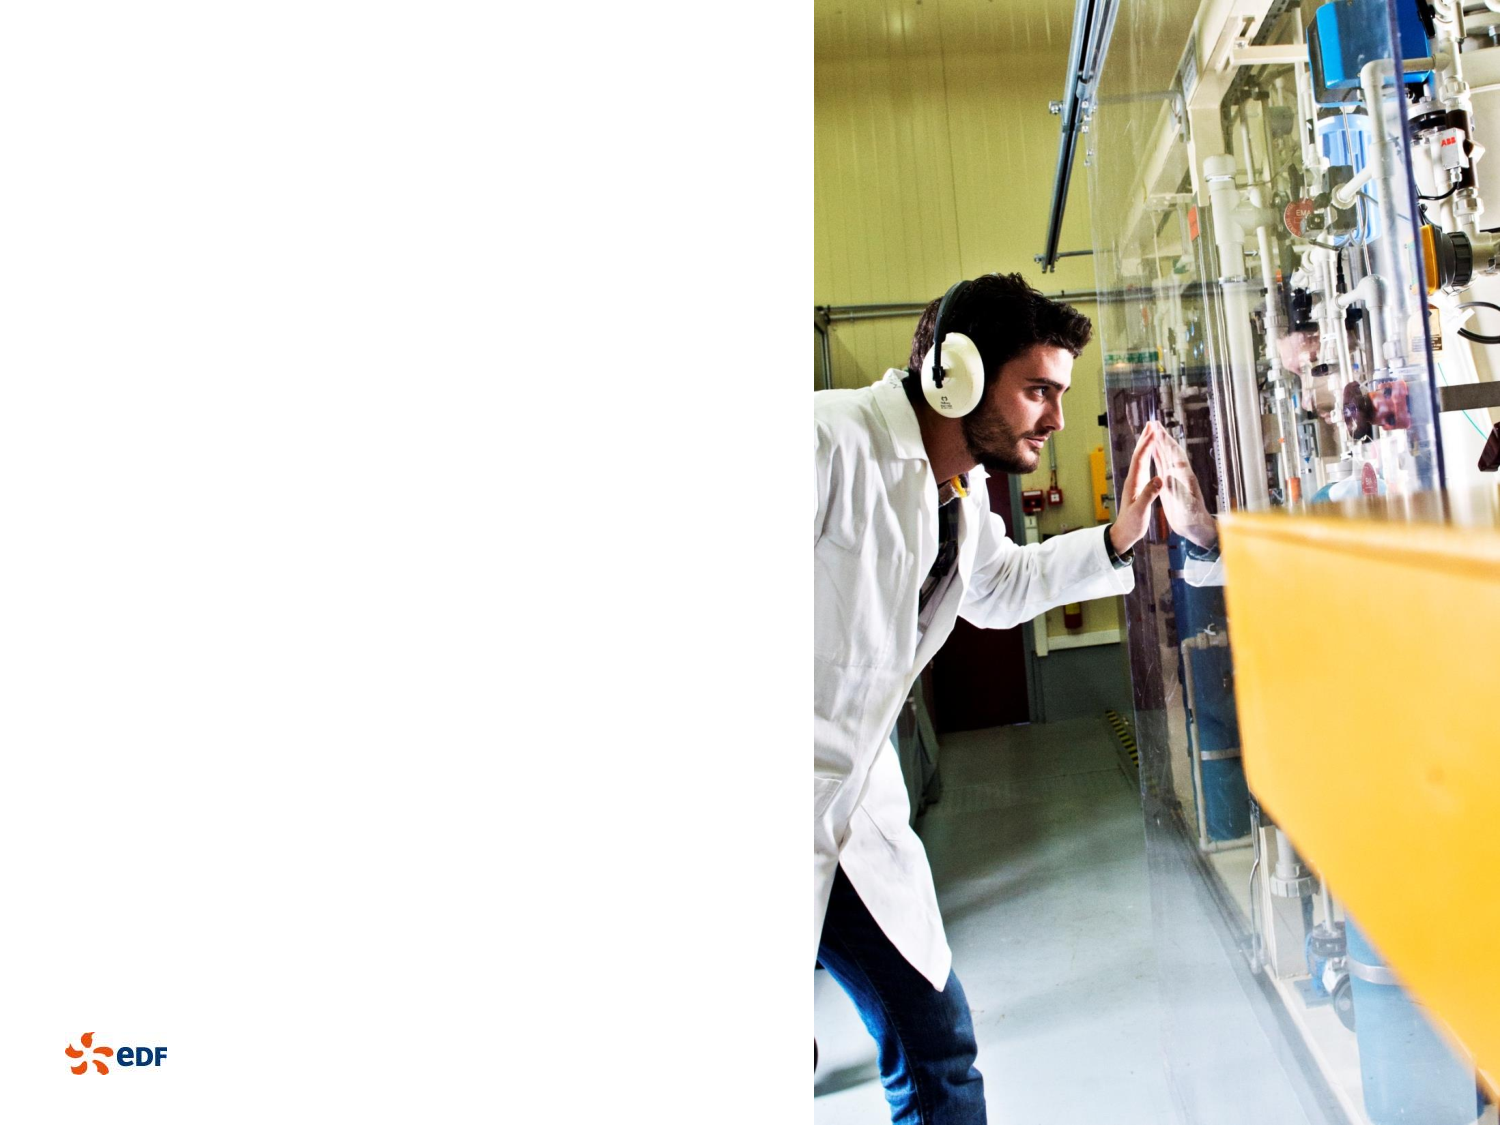
\includepdf{end.pdf}

\begin{frame}[plain]
		\vskip8ex
\begin{columns}[t]
	\begin{column}{5.5cm}
  \titlepage
 % \vspace{5ex}
   \textcolor{gray}{\tiny Copyright  EDF 2020 - Chu Mai (EDF R\&D/MMC)}
  	\end{column}
	\begin{column}{3.2cm}
	  	\end{column}
	  	\end{columns}
\end{frame}



\setbeamertemplate{background canvas}[default]


%%%%%% Table of contents page
%\setbeamertemplate{background canvas}{\pgfuseimage{section_image}}
%  \begin{frame}{Outline}
%\begin{minipage}{6cm}%
%      \tableofcontents[sectionstyle=show/show,subsectionstyle=shade/shade/shade]
%\end{minipage} 
%  \end{frame}
%\addtocounter{framenumber}{-1}
%\setbeamertemplate{background canvas}[default]
%%%%% Table of contents page

%% Body
\part*{} 
\normalsize
\setstretch{1.3}

\begin{frame}{Outline}
  \tableofcontents[sectionstyle=show/show, subsectionstyle=show/show/show]
\end{frame}

\section{Metamodels}

\subsection{Definition, construction and validation}

\begin{frame}[t]{Metamodel - Definition}

\begin{center}
 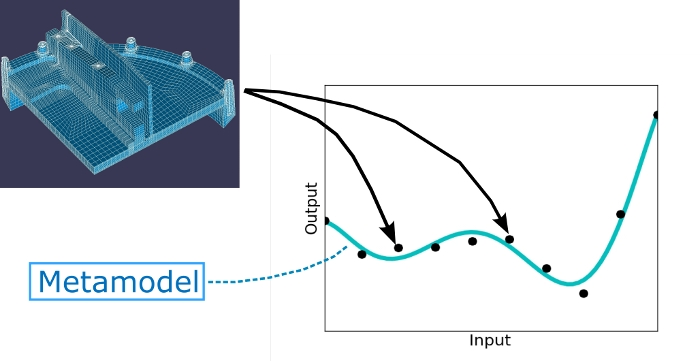
\includegraphics[height=3.2cm]{../Pics/resp_surf_sketch.jpg}
\end{center}


\emph{Meta} : a prefix added to the name of something that consciously references or comments upon its own subject or features, e.g. metamodel : a model of another model

\vspace{0.2cm}
A metamodel is an approximation model that mimics the behaviour of a computationally expensive simulator by training on \emph{observations (data)} of the latter.

 

\end{frame}


\begin{frame}[t]{Metamodel - Definition}

\begin{center}
 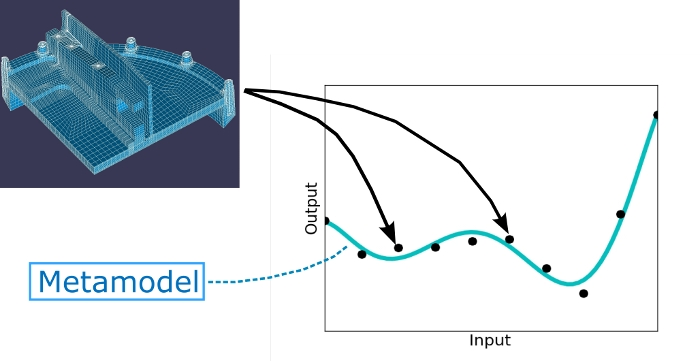
\includegraphics[height=3.2cm]{../Pics/resp_surf_sketch.jpg}
\end{center}


Expensive simulator: $\bs{Y} \; = \; f(\bs{X})$
\begin{itemize}
\item $\bs{X},~\bs{Y}$ are vectors of input and output,
\item $\bs{X}=(X_1,\dots,X_M)$
\end{itemize}
   
Metamodel: $ \widetilde{\bs{Y} } \; = \; \hat{f}(\bs{X}, \bs{\theta})$, $\bs{\theta}$ being its vector of parameters
%\vspace{0.2cm}

By definition, two requirements of a metamodel $\hat{f}$ are:
\begin{itemize}
\item Usefully accurate when predicting away from known observation
\item Being significantly cheaper to evaluate than the primary simulator
\end{itemize}
 

\end{frame}

\begin{frame}[t]{Metamodel - Objectives}

\begin{itemize}
\item Show functional relationships between input parameters and the output quantity of interest: impacts of variables 
\item Augment results from single, expensive simulations: results can be predicted without use of the primary simulator; a continuous predictive function instead of discrete observations
\item Optimize the output quantity of interest: determine configurations that maximize the response or achieve specifications or customer requirements
\item Replace the primary simulator in uncertainty propagation (surrogate model):  sensitivity analysis
%\item Multi-fidelity, multi-level approach: metamodel used as a bridge between a simple but inaccurate code and a more accurate but slower counterpart.
\end{itemize}

\end{frame}

\begin{frame}[t]{Major steps for constructing a metamodel}
 
\begin{center}
 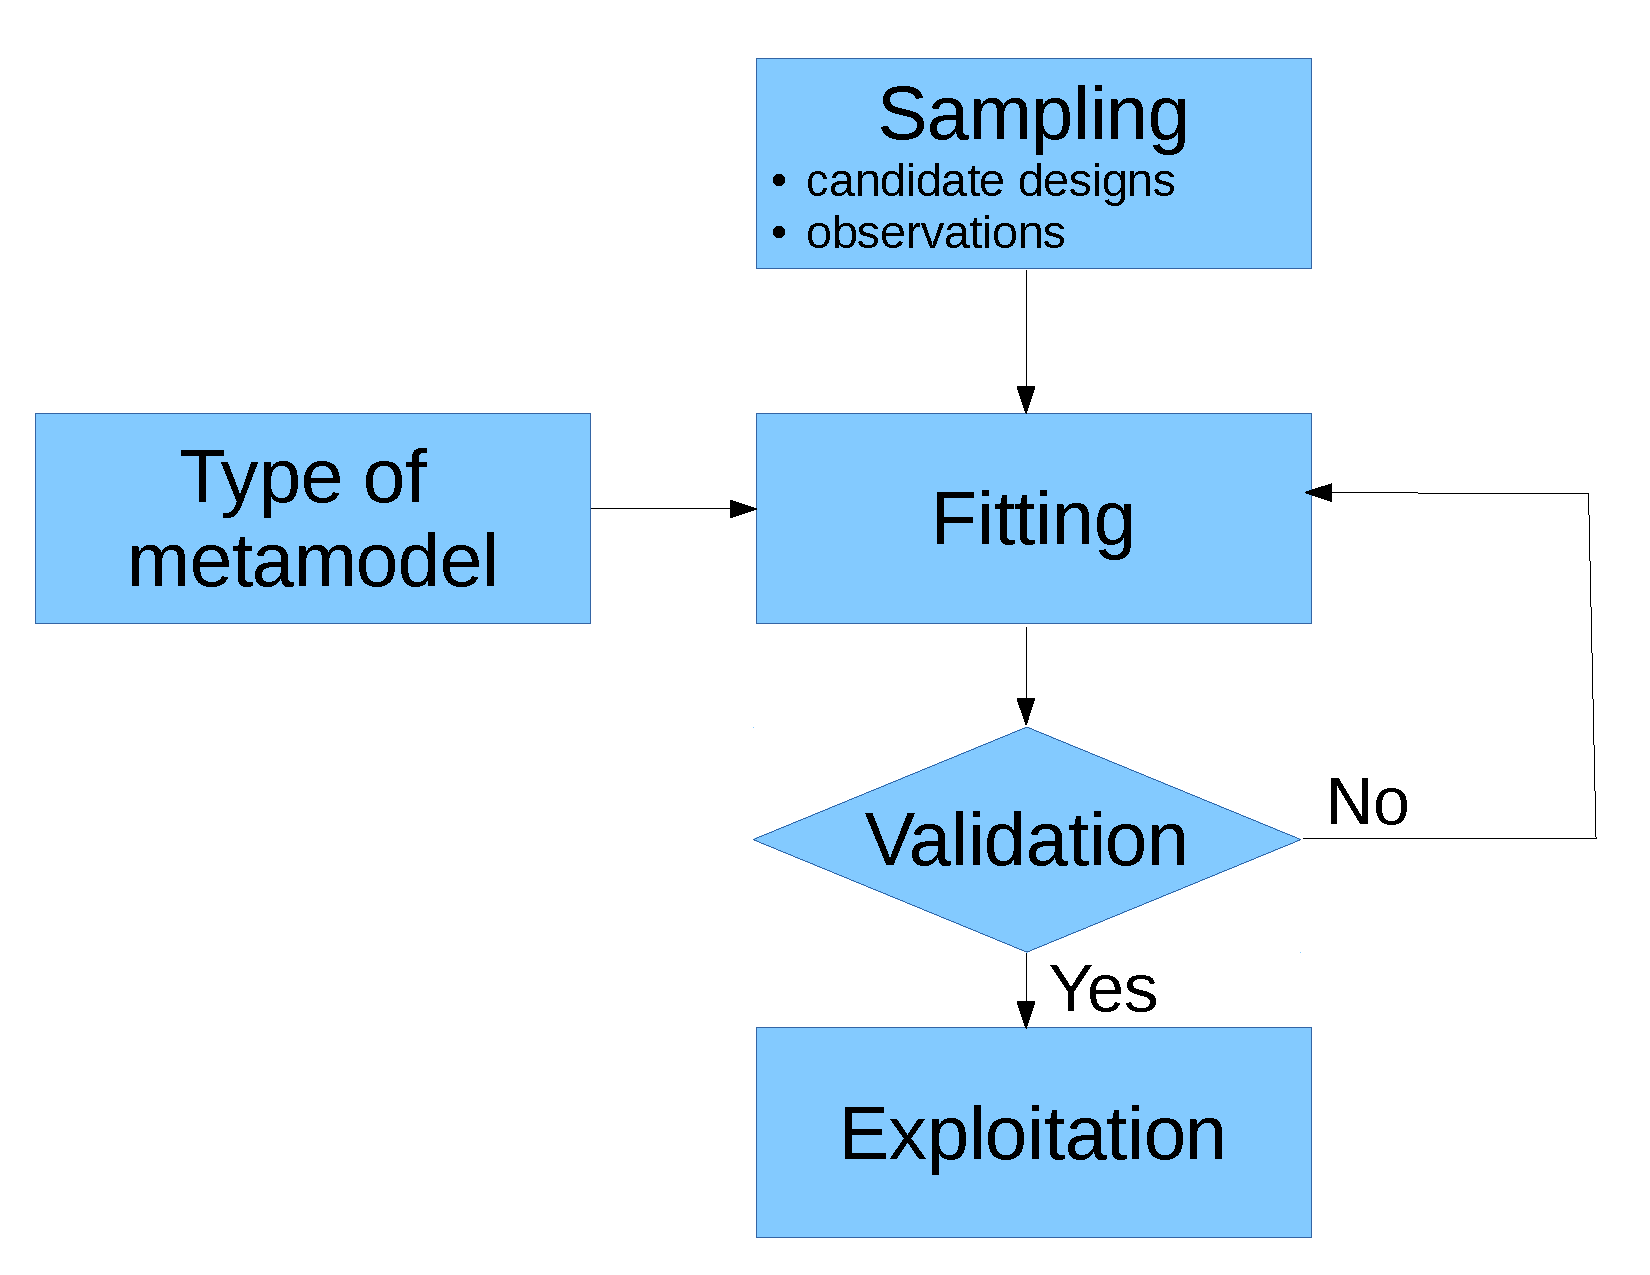
\includegraphics[width=0.8\textwidth]{../Pics/metamodel_scheme.pdf} 
\end{center}

\end{frame}

\begin{frame}[t]{Major steps for constructing a metamodel}

{\titx \bf Sampling (define an experimental design):} 
\begin{itemize}
\item A number of possible candidate designs are generated
\item The designs are launched with the primary simulator
\end{itemize}


{\titx \bf Constructing the metamodel:}
\begin{itemize}
\item A type of metamodel is selected (among several available options)
\item The metamodel is fitted to the available data
\item The metamodel is validated (yes or no)
	\begin{itemize}
	\item if yes: stop
	\item if no, several solutions to be considered
	 \begin{itemize}
	 \item change method for fitting: use advanced regression technique instead of least squares errors,
	 \item change metamodel parameters: increase polynomial degrees,
	 \item enrich the experimental design where the model is inaccurate or interesting behaviour is observed,
	 \item change the type of metamodel: polynomial chaos instead of second-order response surface
	\end{itemize}	     
	\end{itemize}
\end{itemize}

\end{frame}


\begin{frame}[t]{Some types of metamodels}

{\titx \bf Polynomial models:} (response surface)

Second-order model
\[
\tilde{Y} = \theta_0 + \sum_{i=0}^M \, \theta_i \, X_i + \sum_{i=0}^M \, \theta_{ii} \,X_i^2 + \sum_{i<j} \sum_{j=2}^M \theta_{ij} \,X_i \, X_j
\]


{\titx \bf Polynomial chaos expansion:} 
\begin{center}
$\displaystyle{ \tilde{\bs{Y}} }\,  = \, 
\sum_{0 \leq |\bs{k}| \leq p}  \; \theta_{\bs{k}} \psi_{\bs{k}}(\bs{X})  \, $
\end{center}
where $\psi_{\bs{k}}()$ being polynomial chaos functions


{\titx \bf Radial basis function:}
\begin{center}
$\displaystyle{ \tilde{\bs{Y}} }\,  = \, 
\sum_{k = 1}^{N}  \; \theta_{k} \psi( \left\lVert \bs{X} - \bs{X}_k \right\rVert)   $
\end{center}
where $\psi()$ being a radial basis function with its centers taken at $\bs{X}_k$, $k = 1, \dots N$ in the experimental design

\end{frame}

\begin{frame}[t]{Some types of metamodels}

{\titx \bf Kriging:} (Gaussian process regression)

Deterministic trend: linear regression on a fixed basis
\[
m(\bs{X}) = \bs{r(\bs{X})}^T \bs{\theta} 
\]

Random fluctuation: zero-mean stationary Gaussian process of covariance function 
\[
k(\bs{X}, \bs{X'}) = \sigma^2 \, \rho( \left\lVert \bs{X} - \bs{X'}  \right\rVert)
\]


{\titx \bf Artifical neural network:}
Radial basis function is a single layer neural network with radial coordinate neurons
\begin{center}
 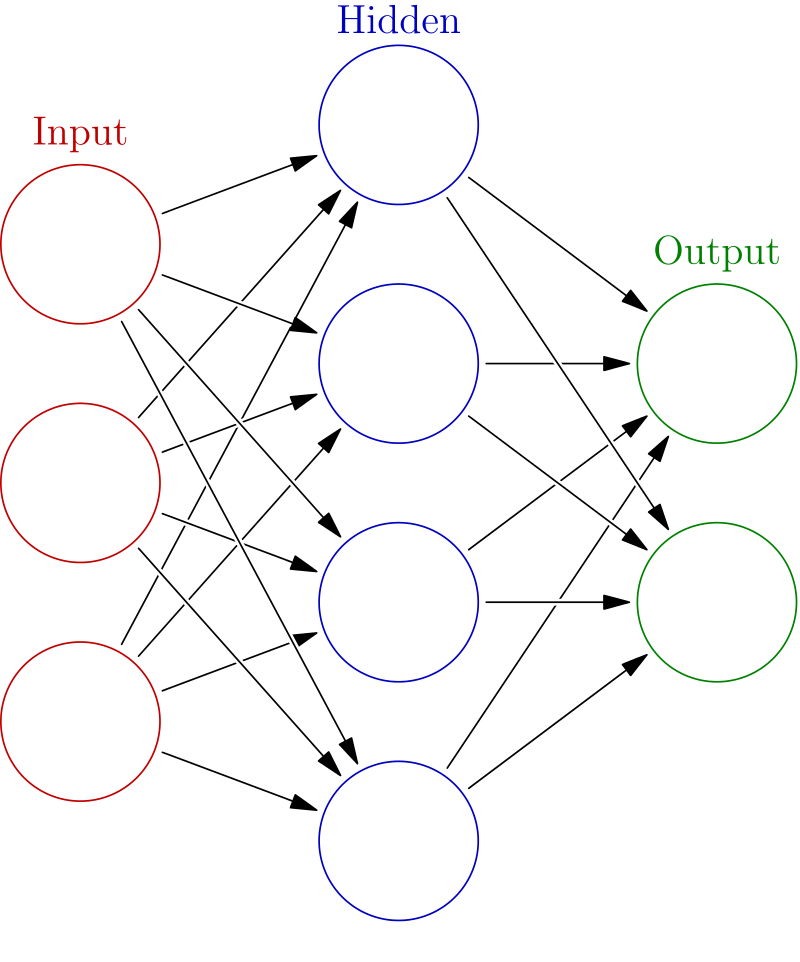
\includegraphics[width=2.8cm]{../Pics/neural_network.png} \\
\end{center}

\end{frame}

\begin{frame}[t]{Methods for fitting metamodels}

{\titx \bf Least square regression:} minimize sum of squared errors of a linear regression model

\[
\bs{\theta}^* = \arg \min_{\bs{\theta}} \, \sum_{i=1}^N \epsilon_i^2 =\arg \min_{\bs{\theta}} \, \sum_{i=1}^N (Y_i - \hat{f}(\bs{X}_i, \bs{\theta}))^2
\]

{\titx \bf Regularized regression methods:} minimize sum of squared errors under a constraint

\[
\bs{\theta}^* = \arg \min_{\bs{\theta}} \, \sum_{i=1}^N (Y_i - \hat{f}(\bs{X}_i, \bs{\theta}))^2 + \lambda \, R(\bs{\theta})
\]

\begin{itemize}
\item $R(\bs{\theta}) = ||\bs{\theta}||_2$: Ridge regression,
\item $R(\bs{\theta}) = ||\bs{\theta}||_1$: LASSO regression,
\item $\lambda$: non-negative regularization coefficient
\end{itemize}
  
\end{frame}

\begin{frame}[t]{Methods for fitting metamodels}

{\titx \bf Maximum likelihood estimation:} e.g. assume that the errors $\epsilon$ are independently randomly distributed according to a normal distribution with standard deviation $\sigma$

\[
\mathcal{L} = \frac{1}{ (2 \pi \sigma^2)^{N/2}} \prod_{i=1}^N exp\left( - \frac{1}{2} \left( \frac{Y_i - \hat{f}(\bs{X}_i, \bs{\theta}) }{\sigma} \right) ^2 \right)
\]

\[
\bs{\theta}^* = \arg \max_{\bs{\theta}} \, \mathcal{L}
\]


{\titx \bf $K$-fold cross-validation method:}

$\mathcal{K}: \{1, \dots , N\} \mapsto \{1, \dots, K\}$ partion of $N$ observations to $K$ roughly equal-sized parts, $K=N$: leave-one-out

$\hat{f}^{-k}()$: fitted metamodel with $k$-th part of data set aside

Cross-validation estimate of prediction error:
\begin{center}
$CV(\hat{f}, \bs{\theta}) = \frac{1}{N} \sum_{i=1}^N L ( Y^i, \hat{f}^{-\mathcal{K}(i)}(X_i) )$
\end{center}

\begin{center}
$
\bs{\theta}^* = \arg \min_{\bs{\theta}} \, CV(\hat{f}, \bs{\theta})
$
\end{center}

 
 
\end{frame}

\begin{frame}[t]{Overfitting}

\begin{center}
 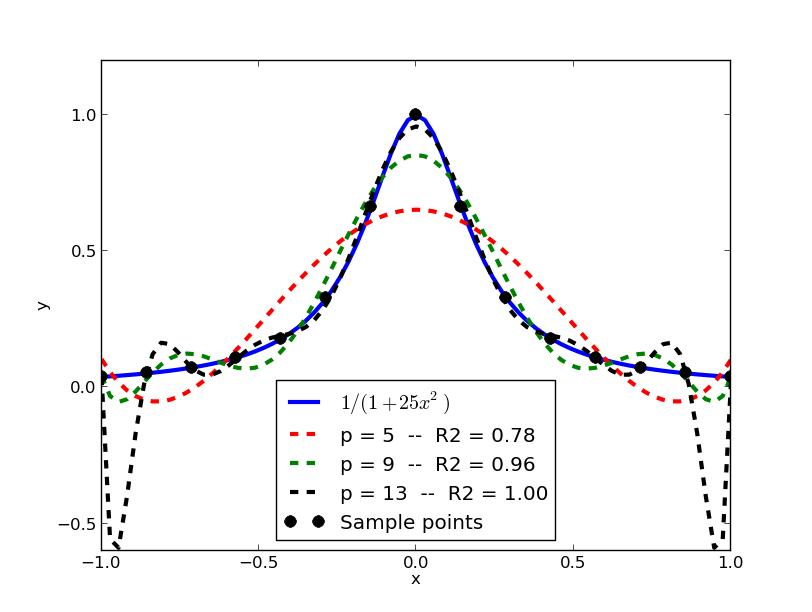
\includegraphics[width=7cm]{../Pics/runge-func-ols.jpeg} \\
\end{center}

\vfill 
\begin{center}
A metamodel that fits closely or exactly a specific set of data (training set) but fails to \emph{predict} future data reliably
\end{center}

\end{frame}

\begin{frame}[t]{Validation of metamodels}

\begin{center}
 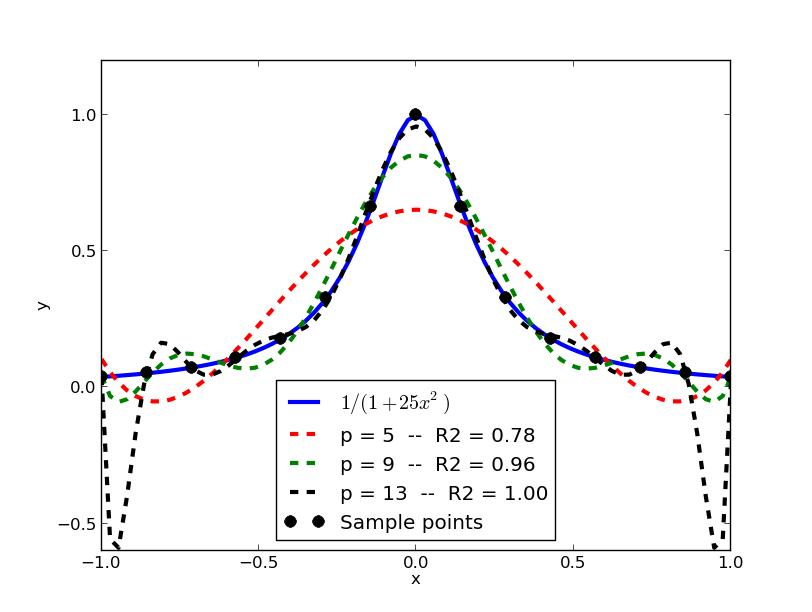
\includegraphics[width=7cm]{../Pics/runge-func-ols.jpeg} \\
\end{center}

\vfill 
Coefficient of determination $R^2$
$$  R^2 \; \; = \; \; 1 - Err \qquad , \qquad Err \quad \propto \quad \sum_{i=1}^N \; \left( f(\xi^{(i)}) - \tilde{f}_{\bs{a}}(\xi^{(i)})  \right)^2  $$

\begin{center}
	$R^2$ does not detect over-fitting and overestimates \emph{predictive} performance
\end{center}

\end{frame}

\begin{frame}[t]{Validation of metamodels}

\begin{center}
 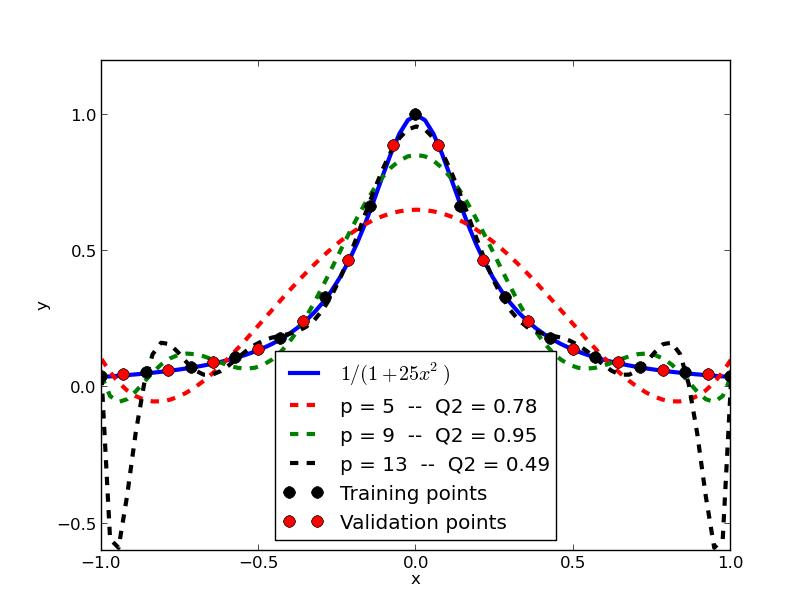
\includegraphics[width=7cm]{../Pics/runge-func-ols-with-q2.jpeg} \\
\end{center}

Equivalent of $R^2$ on an independent validation set:
$$  Q^2 \; \; = \; \; 1 - Err \qquad , \qquad Err \quad \propto \quad \sum_{i=1}^{N_{val}} \; \left( f(\xi^{(i)}) - \hat{f}_{\bs{a}}(\xi^{(i)})  \right)^2  $$

\begin{center}
	Validation on an independent validation set is necessary
\end{center}

\end{frame}

\begin{frame}[t]{Validation of metamodels}

Cross-validation consists in dividing the data sample into two sub-samples. 
\begin{itemize}
	\item A metamodel is built with the first sub-sample (training set)
	\item Its performance is assessed by comparing its predictions with the second sub-sample (test set)
\end{itemize}

Data are often scarce. Partition in training and validation set is a luxury.

\vfill

$K$-fold cross-validation: the data sample is divided into $K$ sub-samples of roughly equal size.

$K= N$: leave-one-out error


%\begin{center}
%$
%\bs{\theta}^* = \arg \min_{\bs{\theta}} \, CV(\hat{f}, \bs{\theta})
%$
%\end{center}

\end{frame}


\subsection{Use for sensitivity analysis}

%\begin{frame}{Probabilistic sensitivity analysis (1)}
%    \small
%    \begin{itemize}
%        \item {\altx Probabilistic modelling:} The uncertain input 
%        parameters are represented by {\altx random variables} with specified 
%        PDF's
%        \item {\altx Uncertainty propagation} through the model
%        ~~~$\longrightarrow$~~~{\altx Random} response
%        \item {\altx \bf Goal:} Evaluate the part of the response variance that 
%        is due to each input~~~$\longrightarrow$~~~{\altx Sobol indices}
%    \end{itemize}
%
%    \begin{center}
%        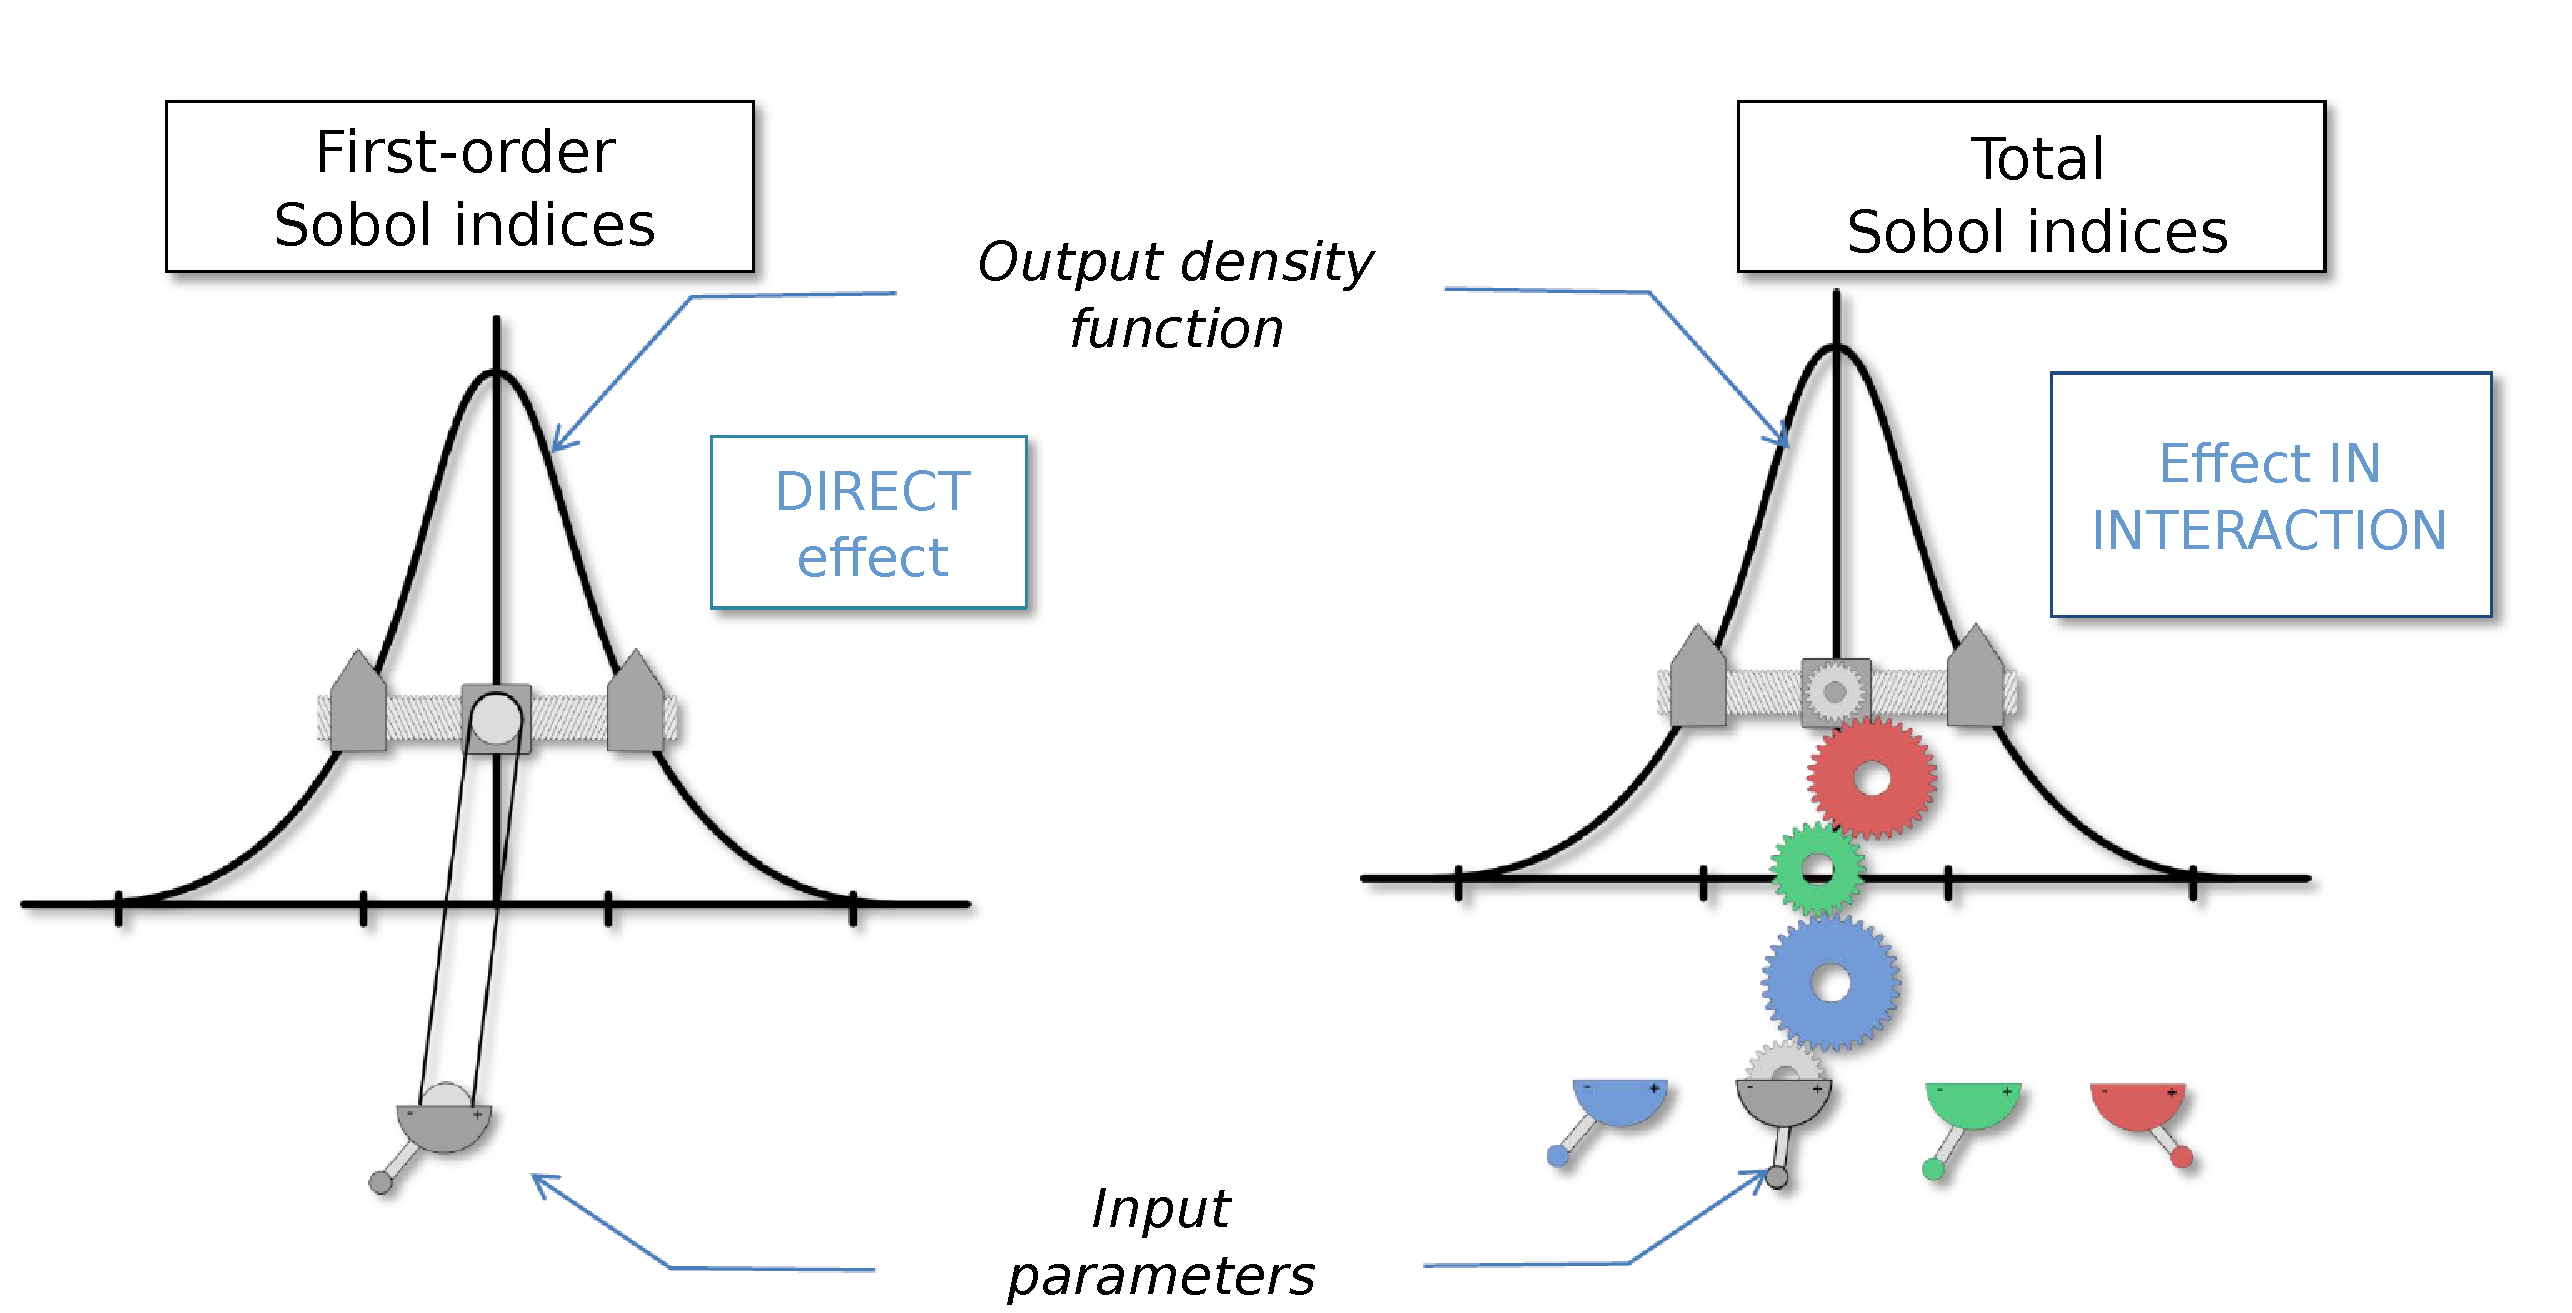
\includegraphics[width=9.5cm]{../Pics/schema_sensibilite.pdf}
%    \end{center}
%
%\end{frame}

\begin{frame}{Variance-based sensitivity analysis}
    \small
    Consider the model $Y=f(\bs{X})$ with random inputs $\bs{X} = \{X_1, \dots, X_M \}$
    \begin{itemize}
        \item The output dispersion is characterized by its {\altx variance} 
        $\V{Y}$
        \item {\altx Partial variance} due to $X_i$: $$\Variance{X_i}{\Expectation{\bs{X} \sim X_i}{Y|X_i}}$$ $\bs{X} \sim X_i$: set of all variables except $X_i$
        \item {\altx Sobol index}, interpretable as a {\altx variance 
        percentage}:
        $${S_i = \frac{\Variance{X_i}{\Expectation{\bs{X} \sim X_i}{Y|X_i}}}{\V{Y}}}$$
        \item Sobol indices to {\altx interactions} can also be defined:
        $${S_{ij} = \frac{\Variance{X_{ij}}{\Expectation{\bs{X} \sim X_{ij}}{Y|X_{ij}}}}{\V{Y}}}$$
    \end{itemize}
    
    \vfill
    
    \begin{center}
        \color{cornellred}{{\bf PROBLEM:} Estimating the partial variances 
        may require many (costly) model evaluations} \\
        
        \vspace{0.3cm}
        {\titx {\bf Solution:} Use an analytic approximation of the model -- 
        {\bf \altx Metamodel}}
    \end{center}

\end{frame}


\section{Polynomial chaos expansion}

\begin{frame}{Polynomial chaos expansion}

Let us consider the model~:~~~$\bs{Y} \; = \; f(\bs{X}) \quad , \quad \bs{X},~ 
\bs{Y}$~~are {\titx random vectors}\\

\begin{center}
 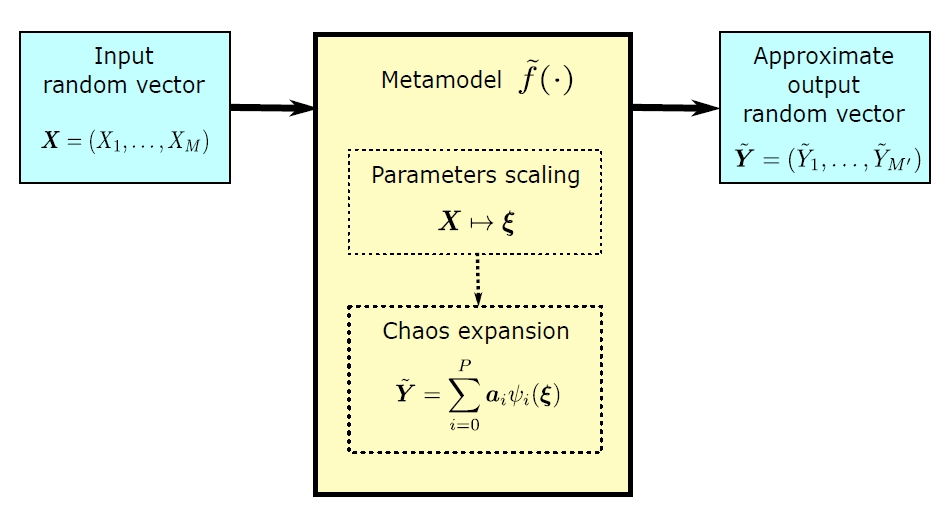
\includegraphics[width=10.5cm]{../Pics/chaos_1.jpg} \\
 
 \vspace{0.2cm}
 
 \color{cornellred}{Decomposition of $Y$ onto an {\titx orthonormal polynomial} basis}
\end{center}

\end{frame}

\begin{frame}{Polynomial chaos basis}

{\titx \bf Assumption:}~~{\titx Independent} input random variables~~$X_1,\dots,
X_M$ \\

\vspace{0.4cm}

{\titx \bf Componentwise transform:}~~$\xi_i \, = \, \mathcal{T}_i(X_i)$~~(often based 
on CDFs, i.e. $\mathcal{T}_i(\cdot) \equiv \mathcal{F}_{\xi_i}^{-1} ( \mathcal{F}_{X_i}(\cdot) )$) \\
\vspace{-0.2cm}
\begin{center}
    \color{cornellred}{---~~~Several possible choices for each $(\xi_i, \mathcal{T}_i)$} \\
    \color{cornellred}{---~~~A given $\xi_i$ dictates the choice of a family 
    $(\pi^{(i)}_k)_{k \geq 0}$ of {\titx orthonormal polynomials}}
\end{center}

\vspace{0.3cm}

Given a uniform random variable $X \sim \mathcal{U}([0,10])$, the transform $\xi = X/5 - 1$ leads to  $\xi \sim \mathcal{U}([-1,1])$ for which {\altx Legendre polynomials} are used:
\[
\pi_0(\xi) = 1 \; \;  ,  \; \; \pi_1(\xi) = \sqrt{3} \xi \; \;  ,  \; \; \pi_2(\xi) = \frac{\sqrt{5}}{2}(3\xi^2-1) \; \;  ,  \; \; \dots 
\]

Given a normal random variable $X \sim \mathcal{N}(5, 1)$, the transform $\xi = X-5$ leads to a standard normal RV $\xi \sim \mathcal{N}(0,1)$ and {\altx Hermite polynomials}:
\[ \pi_0(\xi) = 1 \; \;, \; \; \pi_{1}(\xi) = \xi \; \; , \; \; \pi_2(\xi) = \frac{\sqrt{2}}{2}  \left( \xi^2 - 1 \right) \; \; , \; \; \dots \]

\end{frame}

\begin{frame}[t]{Polynomial chaos basis}

\begin{figure}
\begin{minipage}{.45\textwidth}
\centering
  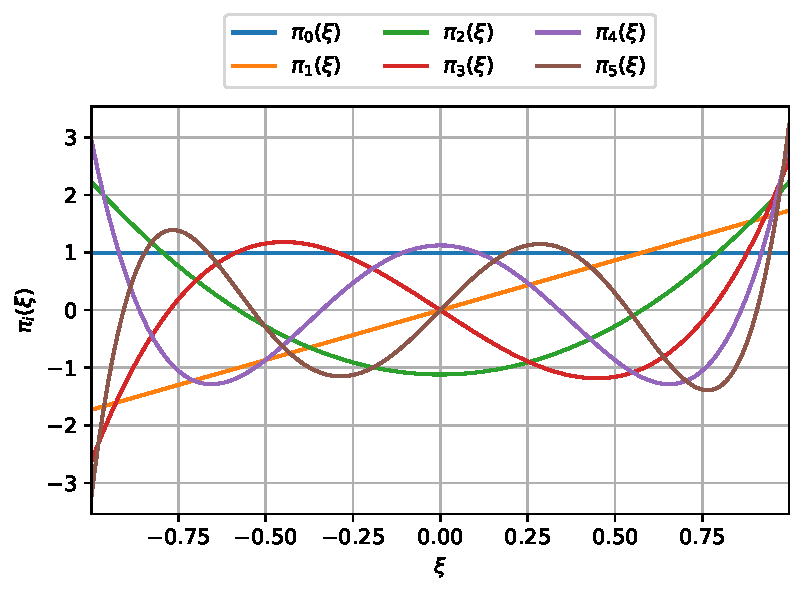
\includegraphics[width=1.0\textwidth]{../Pics/polynomials_uniform.pdf}
  \\
  {Legendre polynomials}
\end{minipage}
\hfill
\begin{minipage}{.45\textwidth}
	\centering
  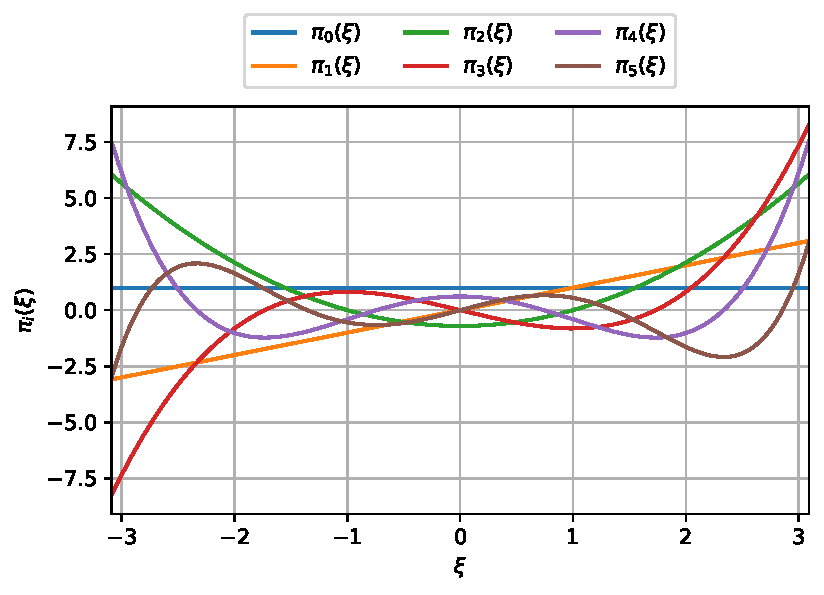
\includegraphics[width=1.0\textwidth]{../Pics/polynomials_normal.pdf}
  \\
  {Hermite polynomials}
\end{minipage}
\end{figure}

{\titx \bf Properties:}~~~~$\pi^{(i)}_0 \, = \, 1 \,, \quad
\E{\pi^{(i)}_k(\xi_i)} \; \equiv \; \; \int_{\mathcal{D}_{\xi}} \; \pi^{(i)}_k(u) \; f_{\xi_i}(u) \; du \; \; = \; \; 0 \, \quad \forall k \geq 1$ \\
\vspace{0.2cm}
~~~~~~~~~~~~~$\E{\pi^{(i)}_k(\xi_i) \; \pi^{(i)}_l(\xi_i)} \equiv \int_{\mathcal{D}_{\xi}} \pi^{(i)}_k(u) \; \pi^{(i)}_l(u) \; f_{\xi_i}(u) \; du \, = \, 
1 \; \; \mbox{ if } \; \; k=l \; \; \mbox{ else } \; \; 0$

\begin{center}
    \color{cornellred}{Relevant for analytical estimation of first-order moments and Sobol' sensitivity indices} \\
\end{center}


\end{frame}


\begin{frame}[t]{Polynomial chaos basis}


{\titx \bf Multivariate orthonormal polynomials:}

\begin{center}
$ \psi_{\bs{k}}(\bs{\xi}) \, = \, 
 \pi^{(1)}_{k_1}(\xi_1) \; 
\times \cdots \times \; \pi^{(M)}_{k_M}(\xi_M)$
\end{center}
$ \bs{\xi} = (\xi_1, \cdots , \xi_M) $: input vector; $ \bs{k} = ( k_1  , \cdots , k_M ) $: indices vector

\vfill
\begin{minipage}{.6\textwidth}
Bivariate Legendre-Hermite polynomials:
{\small \[ \begin{array}{lcl}
\psi_{0,0}(\xi_1,\xi_2) & = & \pi^{(1)}_0(\xi_1) \times \pi^{(2)}_0(\xi_2) = 1  \\
\\
 \psi_{1,0}(\xi_1,\xi_2) & = &\pi^{(1)}_1(\xi_1) \times \pi^{(2)}_0(\xi_2) = \sqrt{3} \xi_1  \\
 \\
 \psi_{1,2}(\xi_1,\xi_2) & = & \pi^{(1)}_1(\xi_1) \times \pi^{(2)}_2(\xi_2) = \frac{\sqrt{6}}{2} \xi_1(\xi_2^2-1) \\
 \end{array} \] }
\end{minipage}
\begin{minipage}{.38\textwidth}
\begin{center}
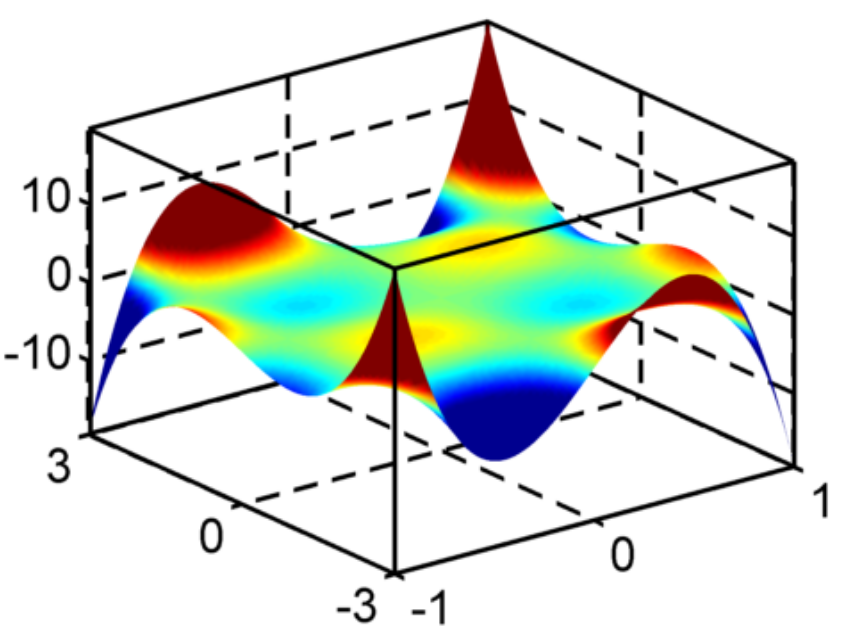
\includegraphics[width=0.8\textwidth]{../Pics/bivariate_polynomial.png}\\
$\psi_{3,3}(\xi_1,\xi_2)$
\end{center}
\end{minipage}

\vfill
{\titx \bf Polynomial chaos expansion:}
\begin{center}
$\displaystyle{ \tilde{\bs{Y}} }\,  = \, 
\sum_{0 \leq |\bs{k}| \leq p}  \; a_{\bs{k}} \psi_{\bs{k}}(\bs{\xi})  \, = \, 
\sum_{0 \leq |\bs{k}| \leq p}  \; a_{\bs{k}} \; \pi^{(1)}_{k_1}(\xi_1) \; 
\times \cdots \times \; \pi^{(M)}_{k_M}(\xi_M)$
\end{center}


\end{frame}


\begin{frame}{Estimation of polynomial chaos coefficients}

\small
\begin{center}
 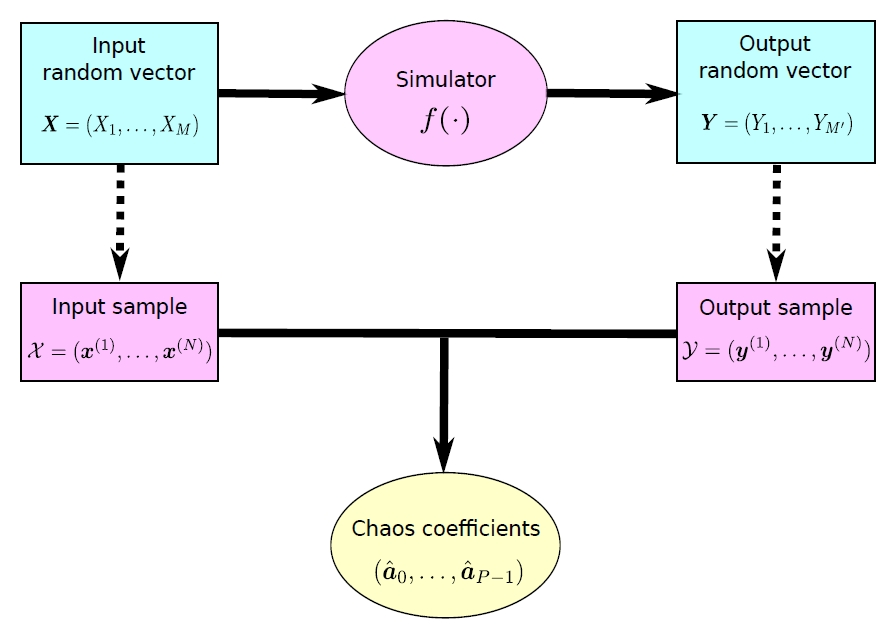
\includegraphics[width=9.5cm]{../Pics/chaos_2.jpg} \\
 \color{cornellred}{{\bf Caution:} the input sample $\mathcal{X}$ must respect the PDF of 
 $\bs{X}$}
\end{center}

\end{frame}

\begin{frame}{Least squares}

\begin{center}
 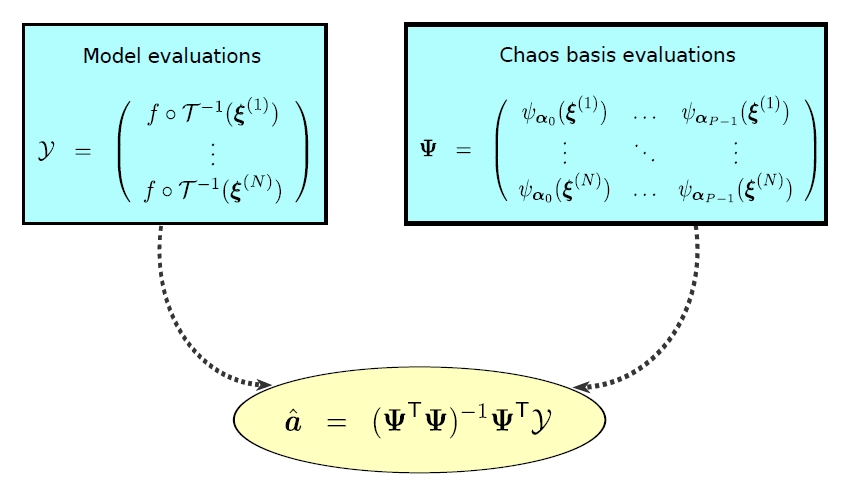
\includegraphics[width=10cm]{../Pics/chaos_3.jpg} \\
 \color{cornellred}{Well-posed problem if $N > P$}
\end{center}

\end{frame}

\begin{frame}{Least angle regression}

\begin{center}
 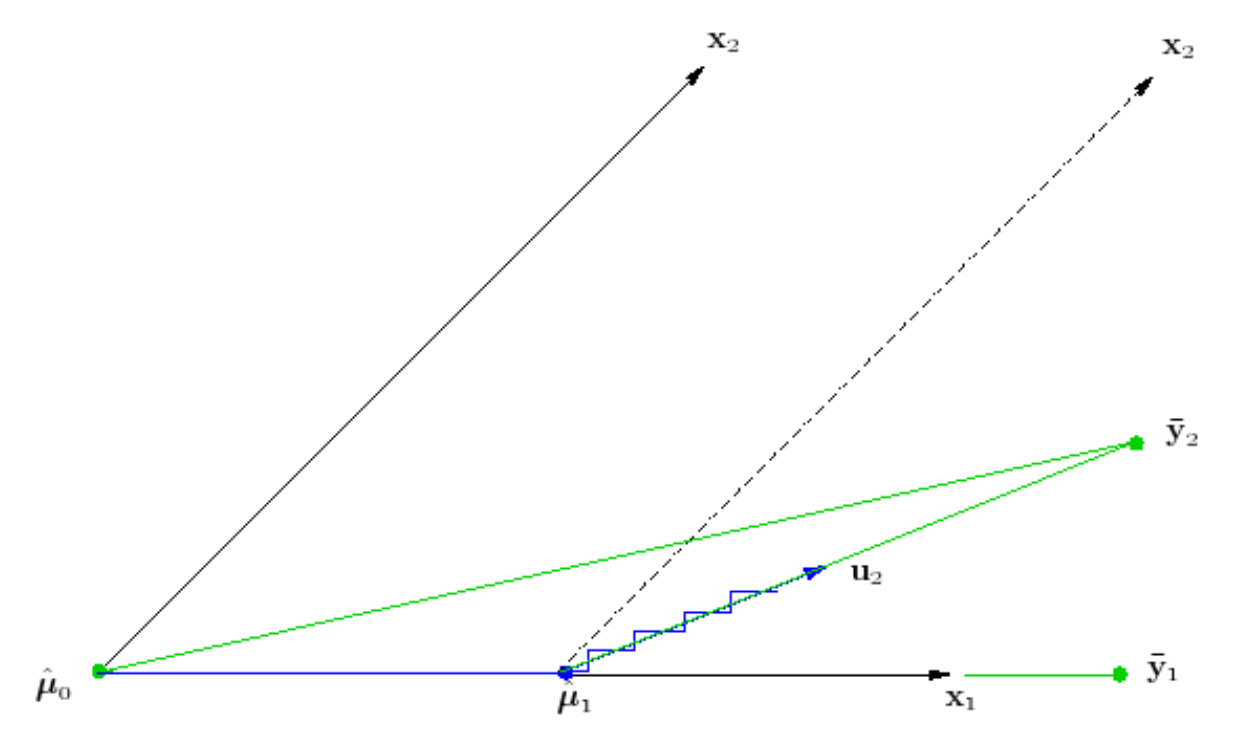
\includegraphics[width=5cm]{../Pics/lars.png} \\
 \color{cornellred}{Least angle regression}
\end{center}

In each iteration:
\begin{itemize}
	\item Find the vector $\psi_{\alpha_j}$ which is as correlated with the current residual as active vectors
	\item Move jointly coefficients until another vector is equi-correlated with the current residual
\end{itemize}

\end{frame}



\begin{frame}[t]{Error indicator}
\begin{itemize}
\item $Q^2$ cross-validation on independent test data set
\item Due to its linear-regression form, leave-one-out error for polynomial chaos expansions can be obtained without calculating $N$ metamodels:
$$  \qquad Err_{L00} \quad = \quad \frac{1}{N} \sum_{i=1}^{N} \; \left( \frac{ f(\xi^{(i)}) - \hat{f}_{\bs{a}}(\xi^{(i)}) } {1 - h_i} \right)^2  $$ 
where $\hat{f}_{\bs{a}}$ is the metamodel computed on the entire data set, $h_i$ is $i$-th diagonal term of the matrix $\boldsymbol{\Psi} \left( \boldsymbol{\Psi}^T \boldsymbol{\Psi} \right)^{-1} \boldsymbol{\Psi}^T$

\end{itemize}





\end{frame}

\begin{frame}{Post-processing: closed-form mean and variance}

\begin{center}
 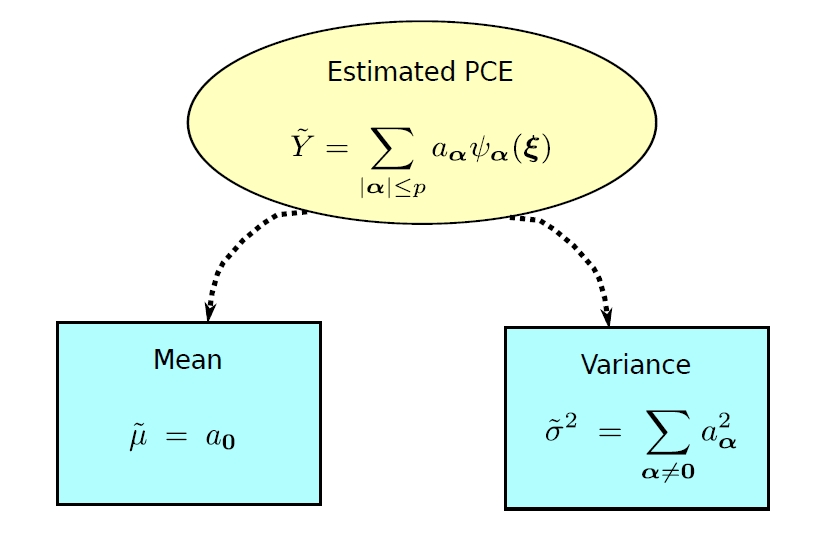
\includegraphics[width=10cm]{../Pics/chaos_4.jpg} 
\end{center}

\end{frame}

\begin{frame}{Post-processing: closed-form Sobol indices}

\begin{center}
 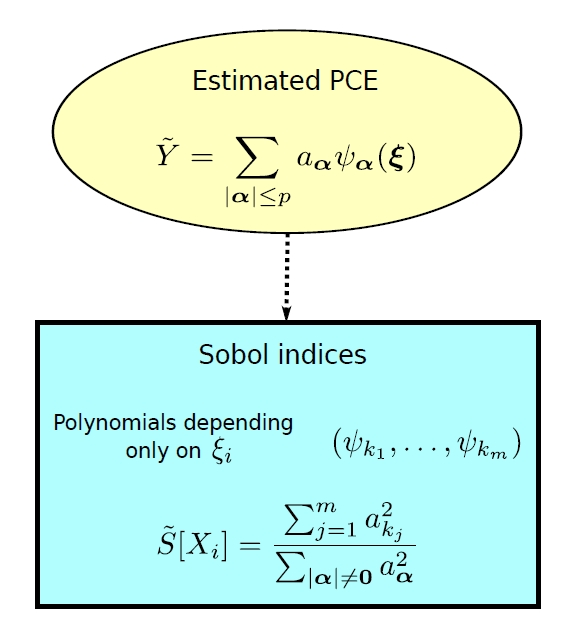
\includegraphics[height=6.5cm]{../Pics/chaos_5.jpg} \\
 \color{cornellred}{Interaction indices can also be derived!}
\end{center}

\end{frame}

\section{Applications in non-destructive testing}

%    \begin{frame}{Context and objectives}
%
%        \small
%        {\altx \bf Context - Nuclear industry:} \\
%        \begin{itemize}
%            \item Required certification of NDTs of primary and secondary circuits 
%            before their on-site implementation            
%            \item Increasing use of {\altx simulation} of ultrasonic {\altx inspections}
%            \item Necessity to have validated codes and reliable input data
%            \item Uncertain knowledge of material properties in a weld
%        \end{itemize}
%
%        \uncover<2->{
%        {\altx \bf Objectives~:} \\
%            \begin{itemize}
%                \item Determine the dispersion of the inspection output due to 
%                input parameter uncertainty
%                \item Identify the parameters with strong or little impact on the 
%                variability
%            \end{itemize}
%        }
%    
%    \end{frame}
    
    \begin{frame}{Primary circuit - Bent tube weld}
    
    \begin{center}
        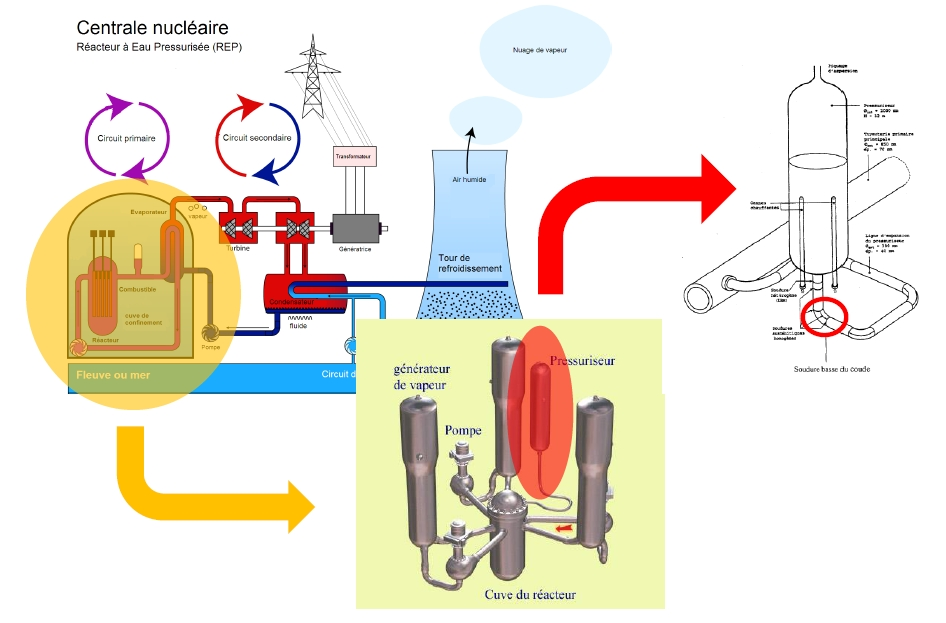
\includegraphics[width=10.4cm]{../Pics/schema_lep.jpg}
    \end{center}
    
    \end{frame}
    
    \begin{frame}{Inspection configuration and modelling}
    
    \begin{center}
        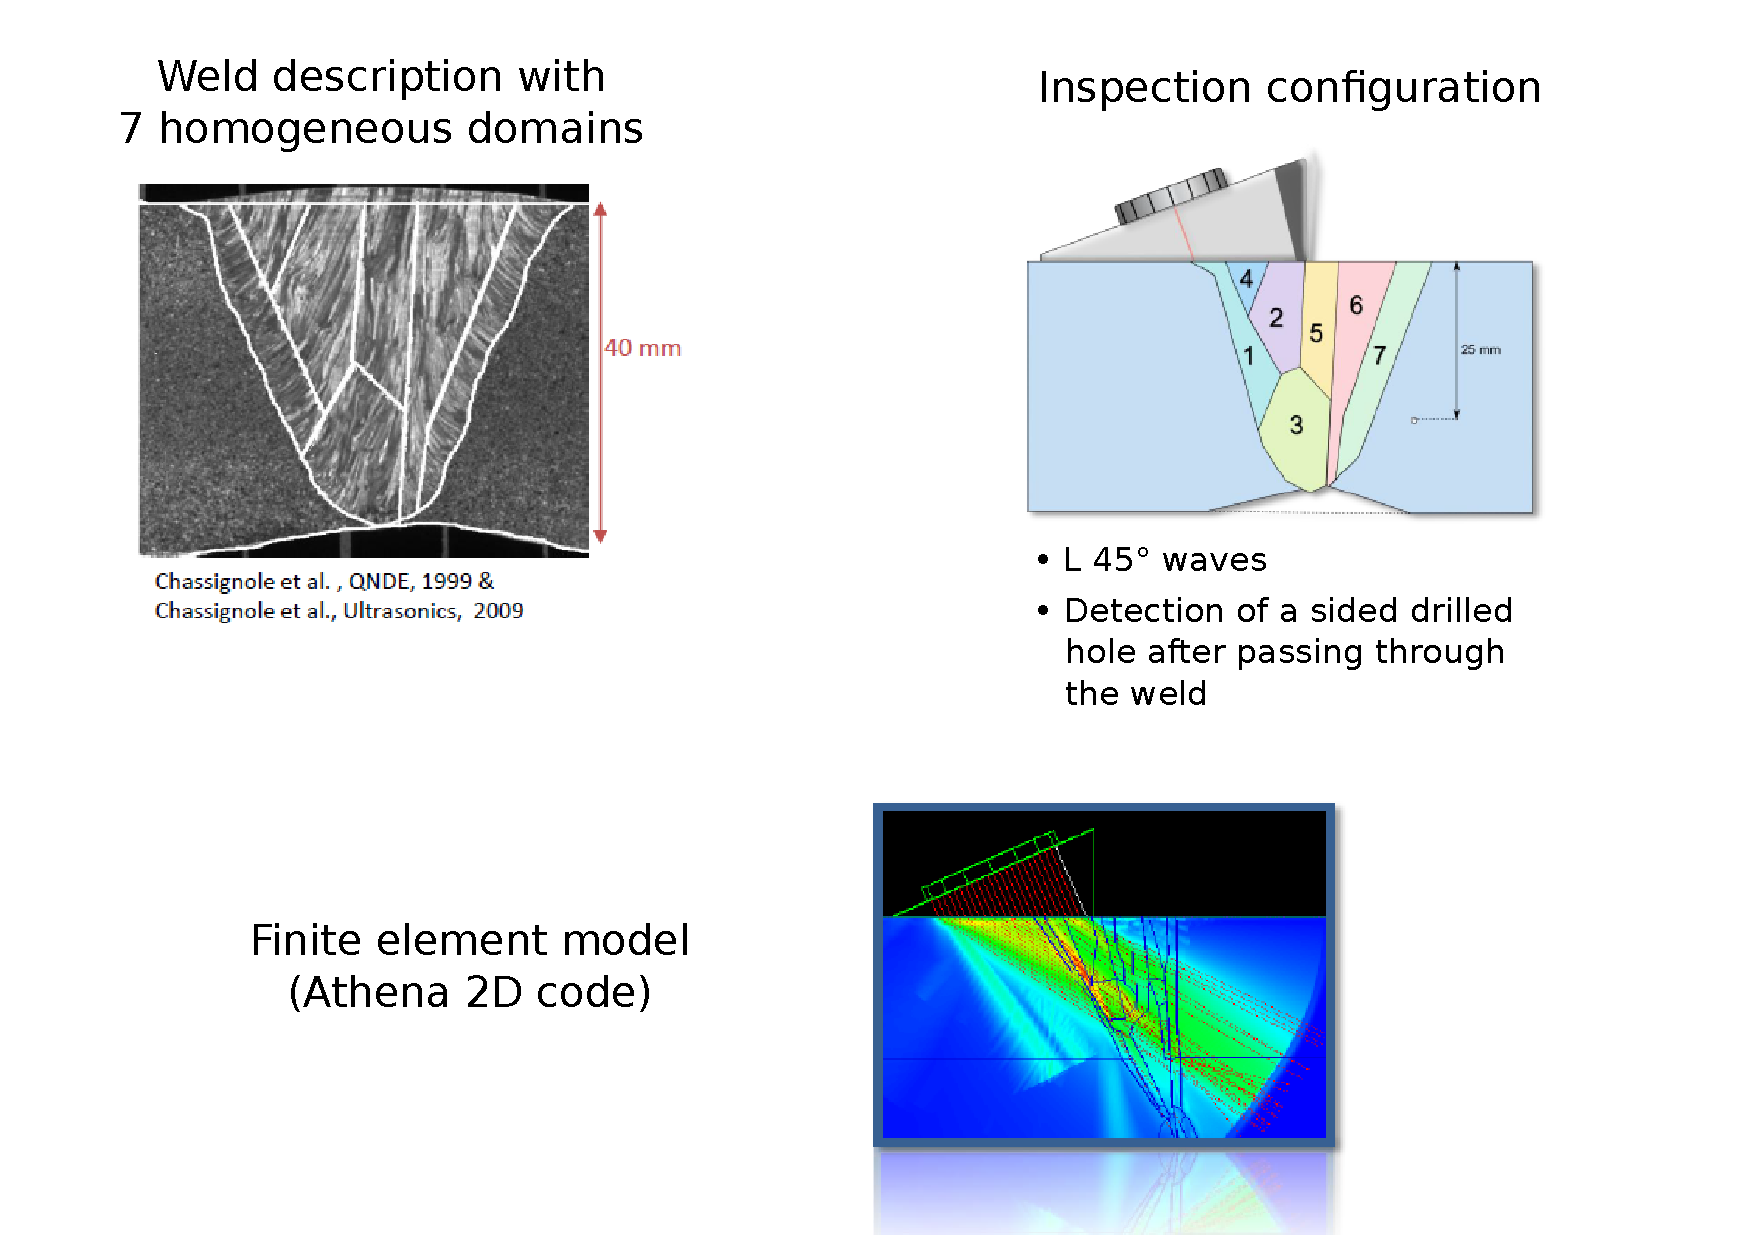
\includegraphics[width=10.4cm]{../Pics/config_controle.pdf}
    \end{center}
    
    \end{frame}
    
    \begin{frame}{Quantities of interest~: inspection results}
    
    \begin{center}
        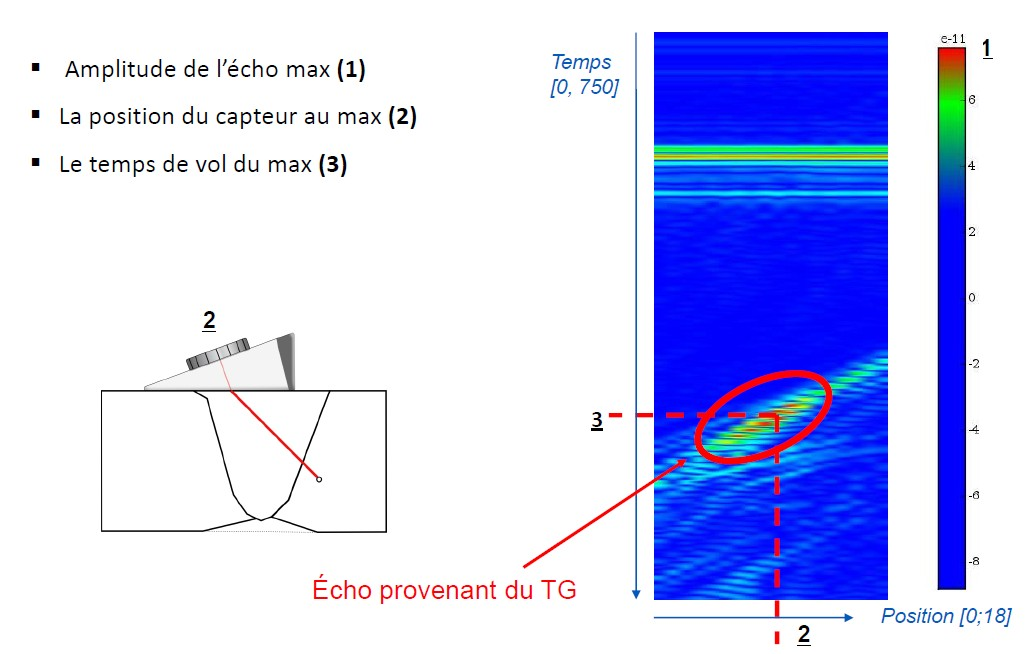
\includegraphics[width=10.8cm]{../Pics/schema_output.jpg}
    \end{center}
    
    \end{frame}
    
    \begin{frame}{Uncertain input data}
    \small
    \begin{center}
        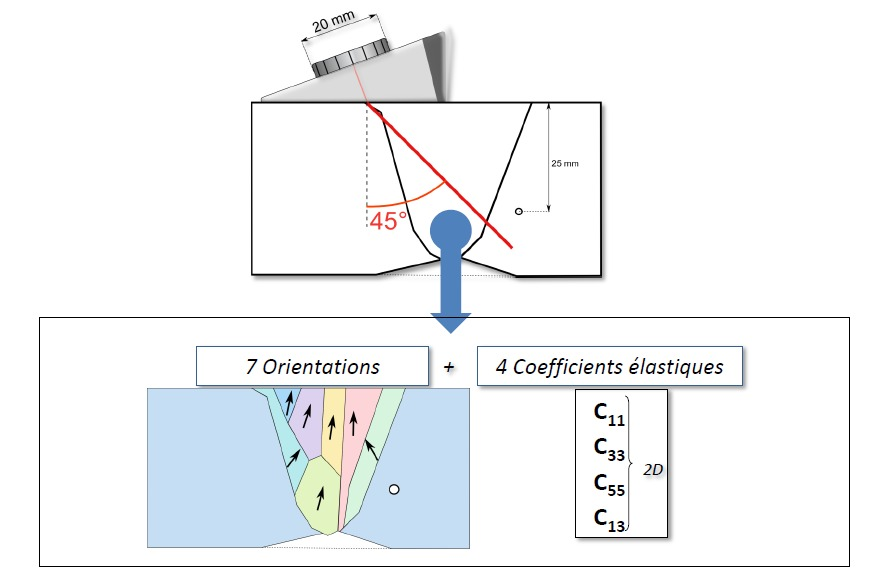
\includegraphics[width=8.5cm]{../Pics/schema_input.jpg} \\
        \vspace{0.3cm}
        {\altx \bf Problem~:} What is the sensitivity of the NDT output to 
        each input parameter? \\
        \vspace{0.1cm}
        {\altx {\bf Strategy:} Evaluate the Sobol sensitivity indices}
    \end{center}
    
    
    \end{frame}
\begin{frame}{Specification of the input PDFs and chaos basis}

    \begin{columns}%[m]
        \begin{column}{5.0cm}
            \begin{center}
            {\small \titx {\bf Input variables:}~~~$X_1,\dots,X_8$ \\
            (independent)}
            \end{center}
        \end{column}
        \begin{column}{5.0cm}
            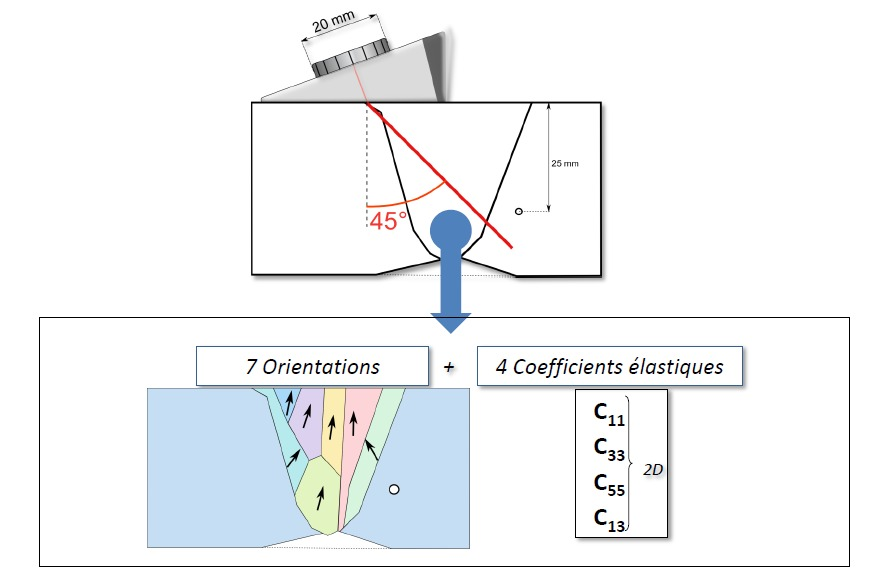
\includegraphics[width=4.5cm]{../Pics/schema_input.jpg}
        \end{column}
    \end{columns}
    
    \vspace{0.3cm}
    
    \scriptsize 
    
    \begin{columns}%[m]
        \begin{column}{5.0cm}
            ~~~~~~~~~~~~~~~~~~~~~~~~~~Elastic constants ($X_1-X_4$)
        \end{column}
        \begin{column}{5.0cm}
            ~~~~~~~~~~Orientations ($X_5-X_{11}$) 
        \end{column}
    \end{columns}
    
    \vspace{-0.3cm}
    
    \begin{center}
        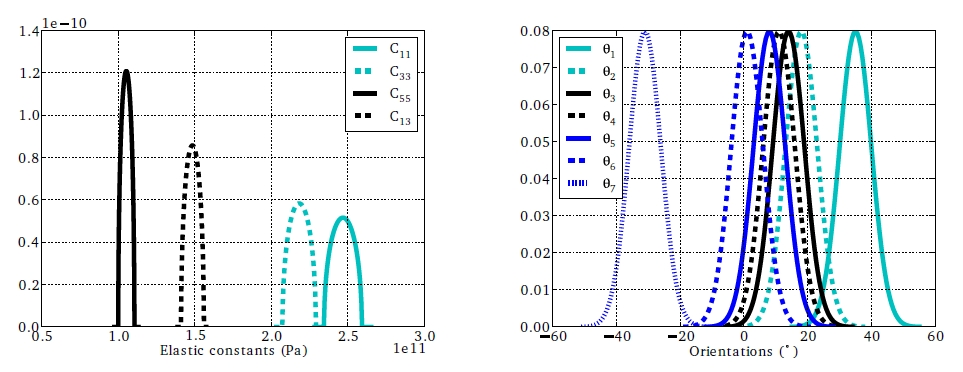
\includegraphics[width=8.5cm]{../Pics/PDFs.jpg} 
    \end{center}
    
    \vspace{-0.1cm}
    
    \begin{columns}%[m]
        \begin{column}{5.0cm}
            ~~~~~~~~~~~~~~~~~~~~~~~~{\titx Beta PDFs} \\
            ~~~~~~~~~~~~~~~~~~~~~~~~~$\xi_i \sim \mathcal{U}(-1,1)$  $\rightarrow$ {\titx Legendre poly.}
        \end{column}
        \begin{column}{5.0cm}
            ~~~~~~~{\titx Normal PDFs} \\
            ~~~~~~~$\xi_i \sim \mathcal{N}(0,1)$  $\rightarrow$ {\titx Hermite poly.}
        \end{column}
    \end{columns}

\end{frame}

\begin{frame}{Construction of the polynomial chaos}
    
    \small
    
    
    \begin{columns}%[m]
        \begin{column}{7.0cm}
            \begin{itemize}
                \item Design of experiments:~~{\titx quasi-random sample} of 
                size $N=2\, 000$
            \end{itemize}
        \end{column}
        \begin{column}{3.5cm}
            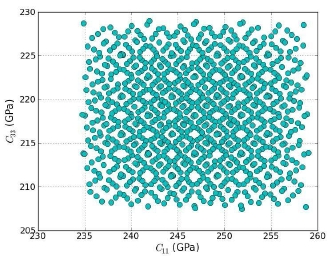
\includegraphics[width=3.5cm]{../Pics/QMC.jpg}
        \end{column}
    \end{columns}
    
    \vspace{0.5cm}
    
    \begin{itemize}
        \item Distributed calls to the FE model (cluster)
    \end{itemize}
    
    \vspace{0.5cm}
    
    \begin{columns}%[m]
        \begin{column}{7.0cm}
            \begin{itemize}
                \item Fit of chaos proxies with varying degree \\
                ~~~~(70\% of the sample points) \\
                ~~~~$\rightarrow$~~optimal degree $p=3$
                \item Validation with the 30\% remaining points
            \end{itemize}
        \end{column}
        \begin{column}{3.5cm}
            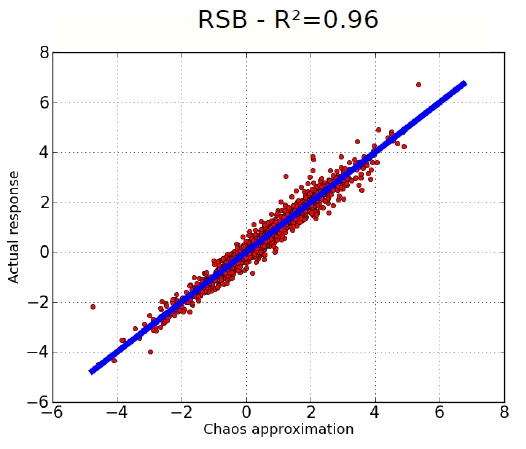
\includegraphics[width=4.0cm]{../Pics/RSB_chaos.jpg}
        \end{column}
    \end{columns}

\end{frame}

\begin{frame}{Sensitivity analysis -- Signal-to-noise ratio}

    \small
    \begin{center}
      \begin{tabular}{m{3.5cm}m{6.0cm}}
        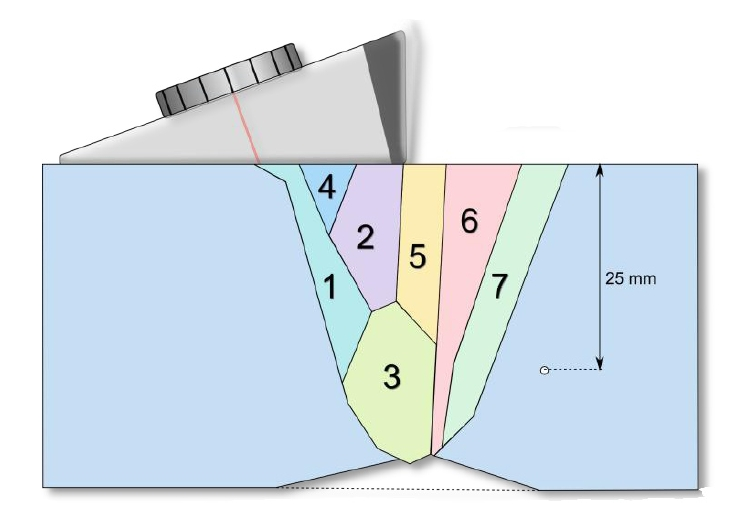
\includegraphics[width=3.5cm]{../Pics/cnd_config.jpg} & 
        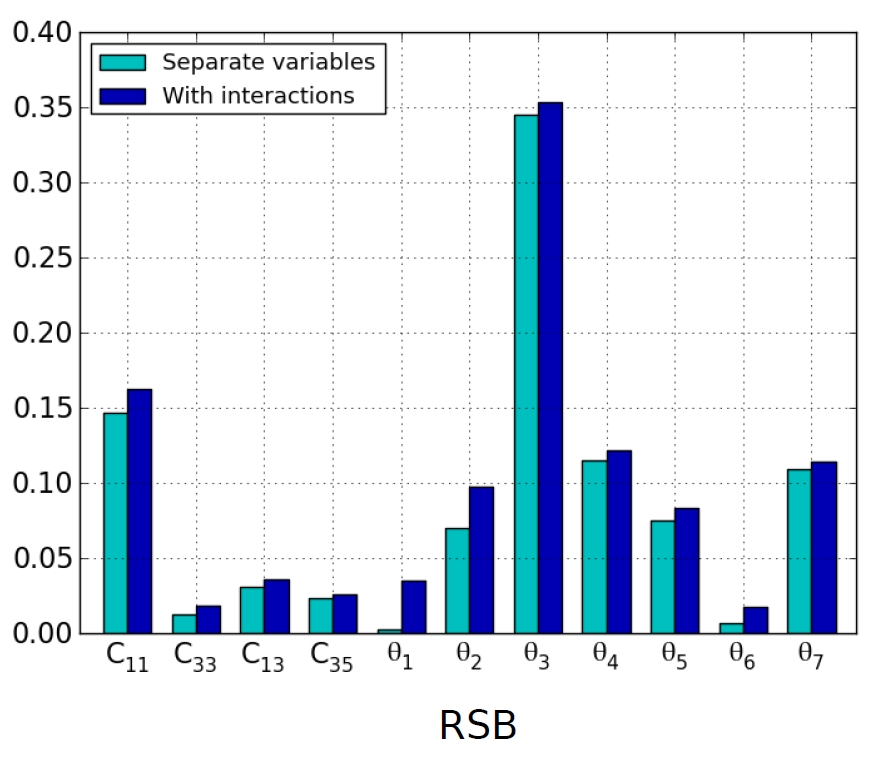
\includegraphics[width=6.0cm]{../Pics/sobol_indices.jpg} \\
      \end{tabular}
        {\titx Almost no interaction effect (additive structure) \\
        Variability mostly due to the orientations (plus $C_{11}$) \\
        $\theta_3$ plays a major role here~~$\rightarrow$~~Check a finer weld 
        description}
    \end{center}

\end{frame}

\section{Conclusions}

\begin{frame}{Metamodels \& Polynomial chaos }

\begin{itemize}
\item For a given problem, ideally test several types of metamodels
\vspace{0.6cm}
\item Polynomial chaos expansion and Kriging are in OpenTurns
\vspace{0.6cm}
\item It is worth assessing carefully the metamodel quality prior to going further
\end{itemize}

\end{frame}


\footnotesize

\pgfdeclareimage[height=1.0\paperheight, width=1.1\paperwidth]{end_image}{end.pdf}
\setbeamertemplate{background canvas}{\pgfuseimage{end_image}}

\begin{frame}[plain]
		\vskip-3ex
\begin{columns}[t]
	\begin{column}{5.5cm}
  \begin{center}
  \textcolor{orange}{\Huge Thank you}
  \end{center}
  	\end{column}
	\begin{column}{3.2cm}
	  	\end{column}
	  	\end{columns}
\end{frame}

\end{document}
